\chapter{สรุปผลการปฎิบัติงาน}
\thispagestyle{empty}
\label{chapter:designAndDevelop}

\titleformat{\paragraph}
{\normalfont\normalsize\bfseries}{\theparagraph}{1em}{}
\titlespacing*{\paragraph}
{0pt}{3.25ex plus 1ex minus .2ex}{1.5ex plus .2ex}

\section{ผลการศึกษาแอปพลิเคชัน HomePro E-Catalog}
โฮมโปร อีแค็ตตาล็อค เป็น แอปพลิเคชันของโฮมโปรที่นำมาใช้ภายในบริษัทไว้ให้พนักงานขายของโฮมโปรที่สาขาสามารถช่วยเพิ่มประสิทธิภาพในการขายได้โดยจะมีเหตุการณ์ที่สามารถช่วยในการ
ขายสามารถมีดังนี้

\subsection{การแสดงสินค้าที่ลูกค้าสนใจ}
    ตัวแอปพลิเคชันสามารถแสดงสินค้าตามที่ผู้ใช้คนหาได้อีกทั้งแบ่งเป็นหมวดแล้วกรองได้หลายวิธี
    ยกตัวอย่างเช่น หากลูกค้าต้องการซื้อโต๊ะทำงานเมื่อลูกค้าถามถึงโต๊ะทำงานพนักงานขายจะเปิดแอปพลิเคชันและทำการแสดงให้ลูกค้าดูแบบของโต๊ะทำงานของที่ {\Company}
    จำหน่ายได้แสดงสีและยีห้อกับราคาตามที่ลูกค้าต้องการอีกทั้ง

\subsection{การแสดงสต๊อคสินค้า}
    ตัวแอปพลิเคชันสามารถแสดงสต๊อคสินค้าของสาขาที่มีสินค้าได้ยกตัวอย่างเช่นหากลูกค้ามาตามหาสินค้าแล้วไม่พบที่ชั้นวางหรือสินค้านี้ในสาขานี้หมดสามารถให้พนักงานเข้าแอปพลิเคชัน
    ค้นหาสินค้าแล้วดูสต๊อคสินค้าของสินค้าที่ต้องการได้ว่าสาขาใดมีบ้างทำให้ไม่เสียลูกค้า

\subsection{การสั่งซื้อสินค้า}
    ตัวสินค้าสามารถสั่งซื้อสินค้าได้เลยเพียงแค่กรอกเบอร์มือถือของลูกค้าก็จะเปรียบเสมือนลูกค้าได้นำสินค้าเข้าตะกร้าทำให้ปิดการขายได้รวดเร็วมากขึ้น

โดยจากการศึกษาแอปพลิเคชันจะสามารถแบ่งมาเป็นเหตุการณ์ (Senario) ในการพัฒนาชุดคำสั่งทดสอบได้ดังนี้
    \begin{enumerate}
        \item หน้า Log-in : กรอกรหัสพนักงาน และ รหัสผ่าน ถูกต้อง
        \item หน้า Log-in : กรอกรหัสพนักงาน หรือ รหัสผ่าน ไม่ถูกต้อง
        \item ออกจากระบบ : ต้องการออกจากระบบด้วยแทบ "ผู้ใช้งาน" ใน BottomNavigationBar
        \item ออกจากระบบ : ต้องการออกจากระบบด้วยแทบ "เมนู" ใน BottomNavigationBar
        \item หน้าหลัก - หมวดหมู่หลัก (Level 3) : ตรวจสอบการแสดงหมวดหมู่สินค้า
        \item หน้าหลัก - หมวดหมู่หลัก (Level 3) : ปุ่มค้นหา
        \item หน้าหลัก - หมวดหมู่ย่อย (Level 2) : ตรวจสอบการแสดงหมวดหมู่สินค้า
        \item หน้าหลัก - หมวดหมู่ย่อย (Level 2) : ดูทั้งหมด
        \item หน้าหลัก - หมวดหมู่ย่อย (Level 1) : เลือกตัวกรอง – ตัวกรองหมวดสินค้า
        \item หน้าหลัก - หมวดหมู่ย่อย (Level 1) : เลือกตัวกรอง – ตัวกรองแบนด์
        \item หน้าหลัก - หมวดหมู่ย่อย (Level 1) : ตรวจสอบการแสดงหมวดหมู่สินค้า Default
        \item หน้าหลัก - หมวดหมู่ย่อย (Level 1) : ตัวเลือก จัดเรียง – เรียงจากราคาน้อยไปหามาก
        \item หน้าหลัก - หมวดหมู่ย่อย (Level 1) : ตัวเลือก จัดเรียง – เรียงจากราคามากไปหาน้อย
        \item หน้าหลัก - หมวดหมู่ย่อย (Level 1) : ตัวเลือก เปรียบสินค้าหน้าหลัก
        \item หน้าหลัก - รายละเอียดสินค้า (Detail) : ปุ่มเปรียบเทียบ หน้า Detail
        \item หน้าหลัก - รายละเอียดสินค้า (Detail) : แถบรายละเอียดสินค้า
        \item หน้าหลัก - รายละเอียดสินค้า (Detail) : แถบข้อมูลจำเพาะ
        \item หน้าหลัก - รายละเอียดสินค้า (Detail) : แทบโปรโมชั่นหน้าหลัก
        \item หน้าหลัก - รายละเอียดสินค้า (Detail) : ปุ่ม สต๊อกสินค้า
        \item หน้าหลัก - รายละเอียดสินค้า (Detail) : ปุ่ม สต๊อกสินค้าเพิ่มเติม
        \item หน้าจอเปรียบเทียบสินค้า : เปรียบเทียบ
        \item หน้าจอเปรียบเทียบสินค้า : เปรียบเทียบมากกว่า 3 รายการ
        \item หน้าจอเปรียบเทียบสินค้า : ยกเลิกตัวที่เปรียบเทียบบางรายการ
        \item หน้าจอเปรียบเทียบสินค้า : ยกเลิกการเปรียบเทียบทั้งหมด
        \item หน้าจอเปรียบเทียบสินค้า : ปุ่ม เพิ่มลงรถเข็น
        \item รถเข็นสินค้า – แก้ไขรายการสินค้า : แก้ไขจำนวนสินค้า (เพิ่ม-ลด)
        \item รถเข็นสินค้า – แก้ไขรายการสินค้า : แก้ไขจำนวนสินค้า (เพิ่ม) โดยให้มี QTY รวมกันเกิน 999
        \item รถเข็นสินค้า – แก้ไขรายการสินค้า : ลบรายการสินค้า
        \item รถเข็นสินค้า – สร้างใบคำสั่งซื้อ : สร้างใบคำสั่งซื้อ โดยใช้เบอร์โทรที่ไม่ใช่เบอร์มือถือ
        \item รถเข็นสินค้า – สร้างใบคำสั่งซื้อ : สร้างใบคำสั่งซื้อ โดยใช้เบอร์โทรที่เบอร์มือถือถูกต้อง
        \item ผู้ใช้งาน : ข้อมูลผู้เข้าใช้งาน
        \item เมนู – เลือกหมวดสินค้า : การค้นหาสินค้าจากการเลือกหมวดสินค้า
        \item เมนู – เลือกตามแบรนด์ : การค้นหาสินค้าจากการเลือกแบรนด์สินค้า
        \item เมนู – ภาษา : การเลือกภาษา
    \end{enumerate}

\newpage
\section{ผลการทดสอบด้วยกรจับ Element บนหน้าจอโดยไม่ต้องแก้ไขที่ Source Code}
% \section{โครงสร้างของระบบ}
% การพัฒนาส่วนการจองซื้อหุ้นกู้สำหรับแอปพลิเคชัน ซีไอเอ็มบีไทยดิจิตอลแบงก์กิ้ง มีการพัฒนาทั้งบนระบบปฏิบัติการ Android โดยใช้ภาษา Kotlin
% และบนระบบปฏิบัติการ iOS โดยใช้ภาษา Swift อีกทั้งยังมีการใช้รูปแบบการพัฒนาแอปพลิเคชันแบบ Super App และ Mini App
% เพื่อที่จะทำให้แต่ละทีมสามารถพัฒนาไปพร้อมกันได้โดยไม่เกิดการขัดกัน โดยส่วนต่าง ๆ ในแอปพลิเคชันจะเป็น Mini App และจะถูกรวบรวมเอาไว้ที่
% Super App เพื่อเป็นแอปพลิเคชันที่สมบูรณ์ดังรูปที่ \ref{super-app-mini-app} โดย Super App จะมอง Mini App ทั้งหมดเป็น Dependencies 
% ที่ Super App ต้องเรียกใช้เพื่อให้แอปพลิเคชันทำงานได้โดยแต่ละ Mini App ก็ต้อง Export ตัวเองออกมาให้เป็น Library ซึ่งแต่ละทีมแยกกันทำงานได้
% โดยไม่ขัดกันดังที่กล่าวไว้ข้างต้น
% \begin{figure}[H]
%     \centering
%     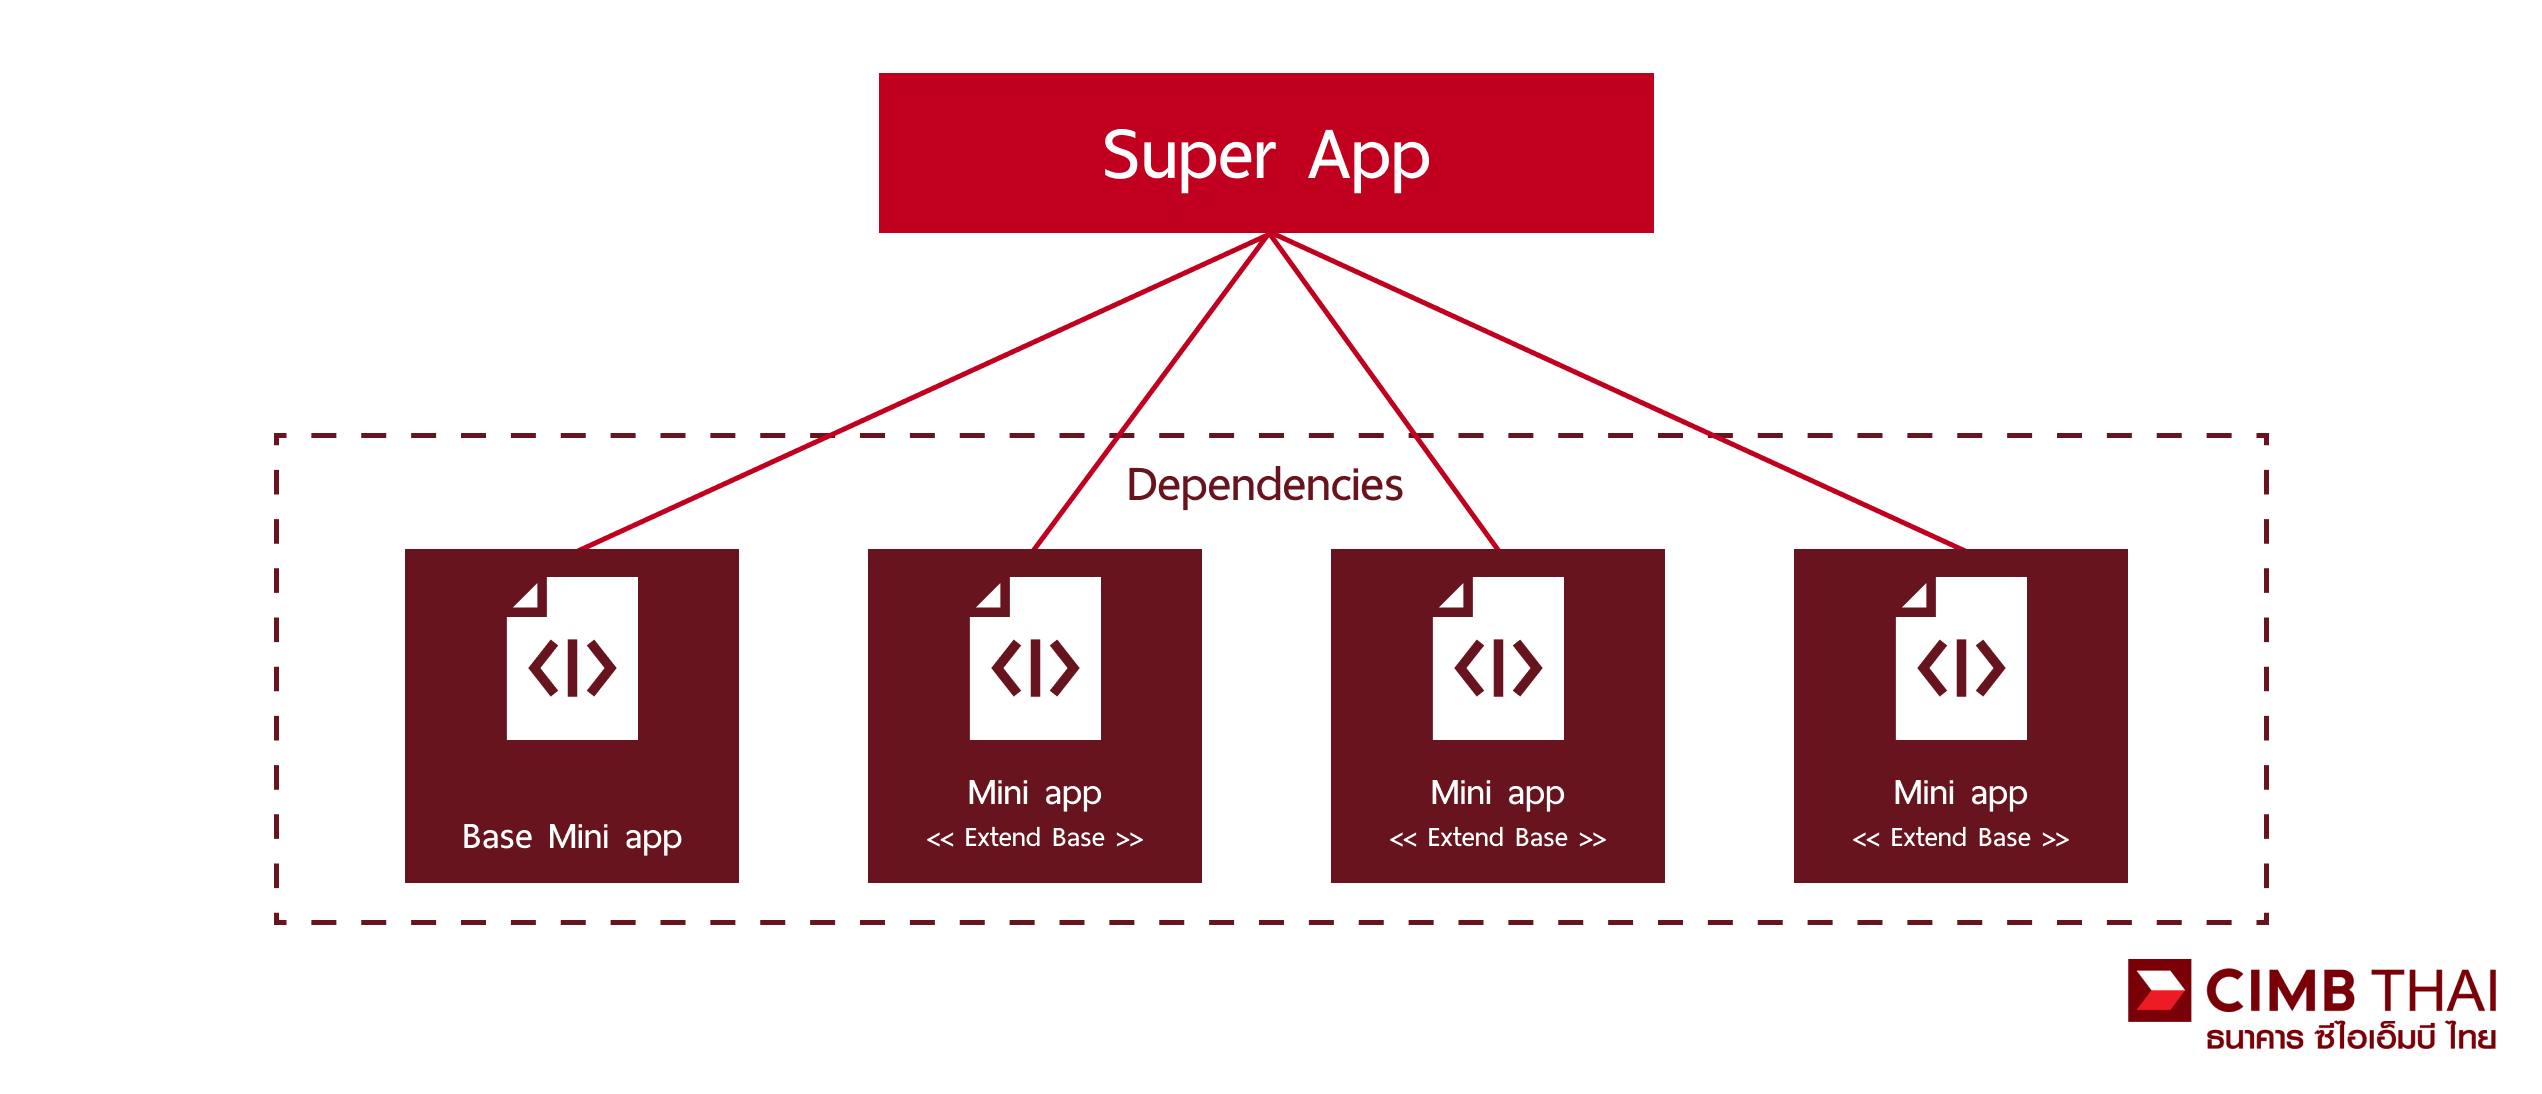
\includegraphics[width=1\textwidth]{super-app-mini-app}
%     \caption{โครงสร้างการพัฒนาแอปพลิเคชันรูปแบบ Super App และ Mini App}\label{super-app-mini-app}
% \end{figure}

% ส่วนเว็บไซต์การจัดการข้อมูลหุ้นกู้ใช้ภาษา Python ในการพัฒนาโดยใช้ประโยชน์จาก Django Framework เข้า
% มาแบ่งแยกส่วนต่าง ๆ เพื่อให้ตอบสนองการทำงานเป็นทีมได้ดีขึ้น และยังมีส่วนของภาษา JavaScript ที่ใช้ประโยชน์จาก Vue.js
% เข้ามาเป็นตัวควบคุมข้อมูลกับ API และสุดท้ายในส่วนของ API นั้นพัฒนาด้วยภาษา Java ซึ่งใช้ประโยชน์จาก Spring Boot Framework
% โดยมีโครงสร้างระบบดังรูปที่ \ref{app-structure}
% \begin{figure}[H]
%     \centering
%     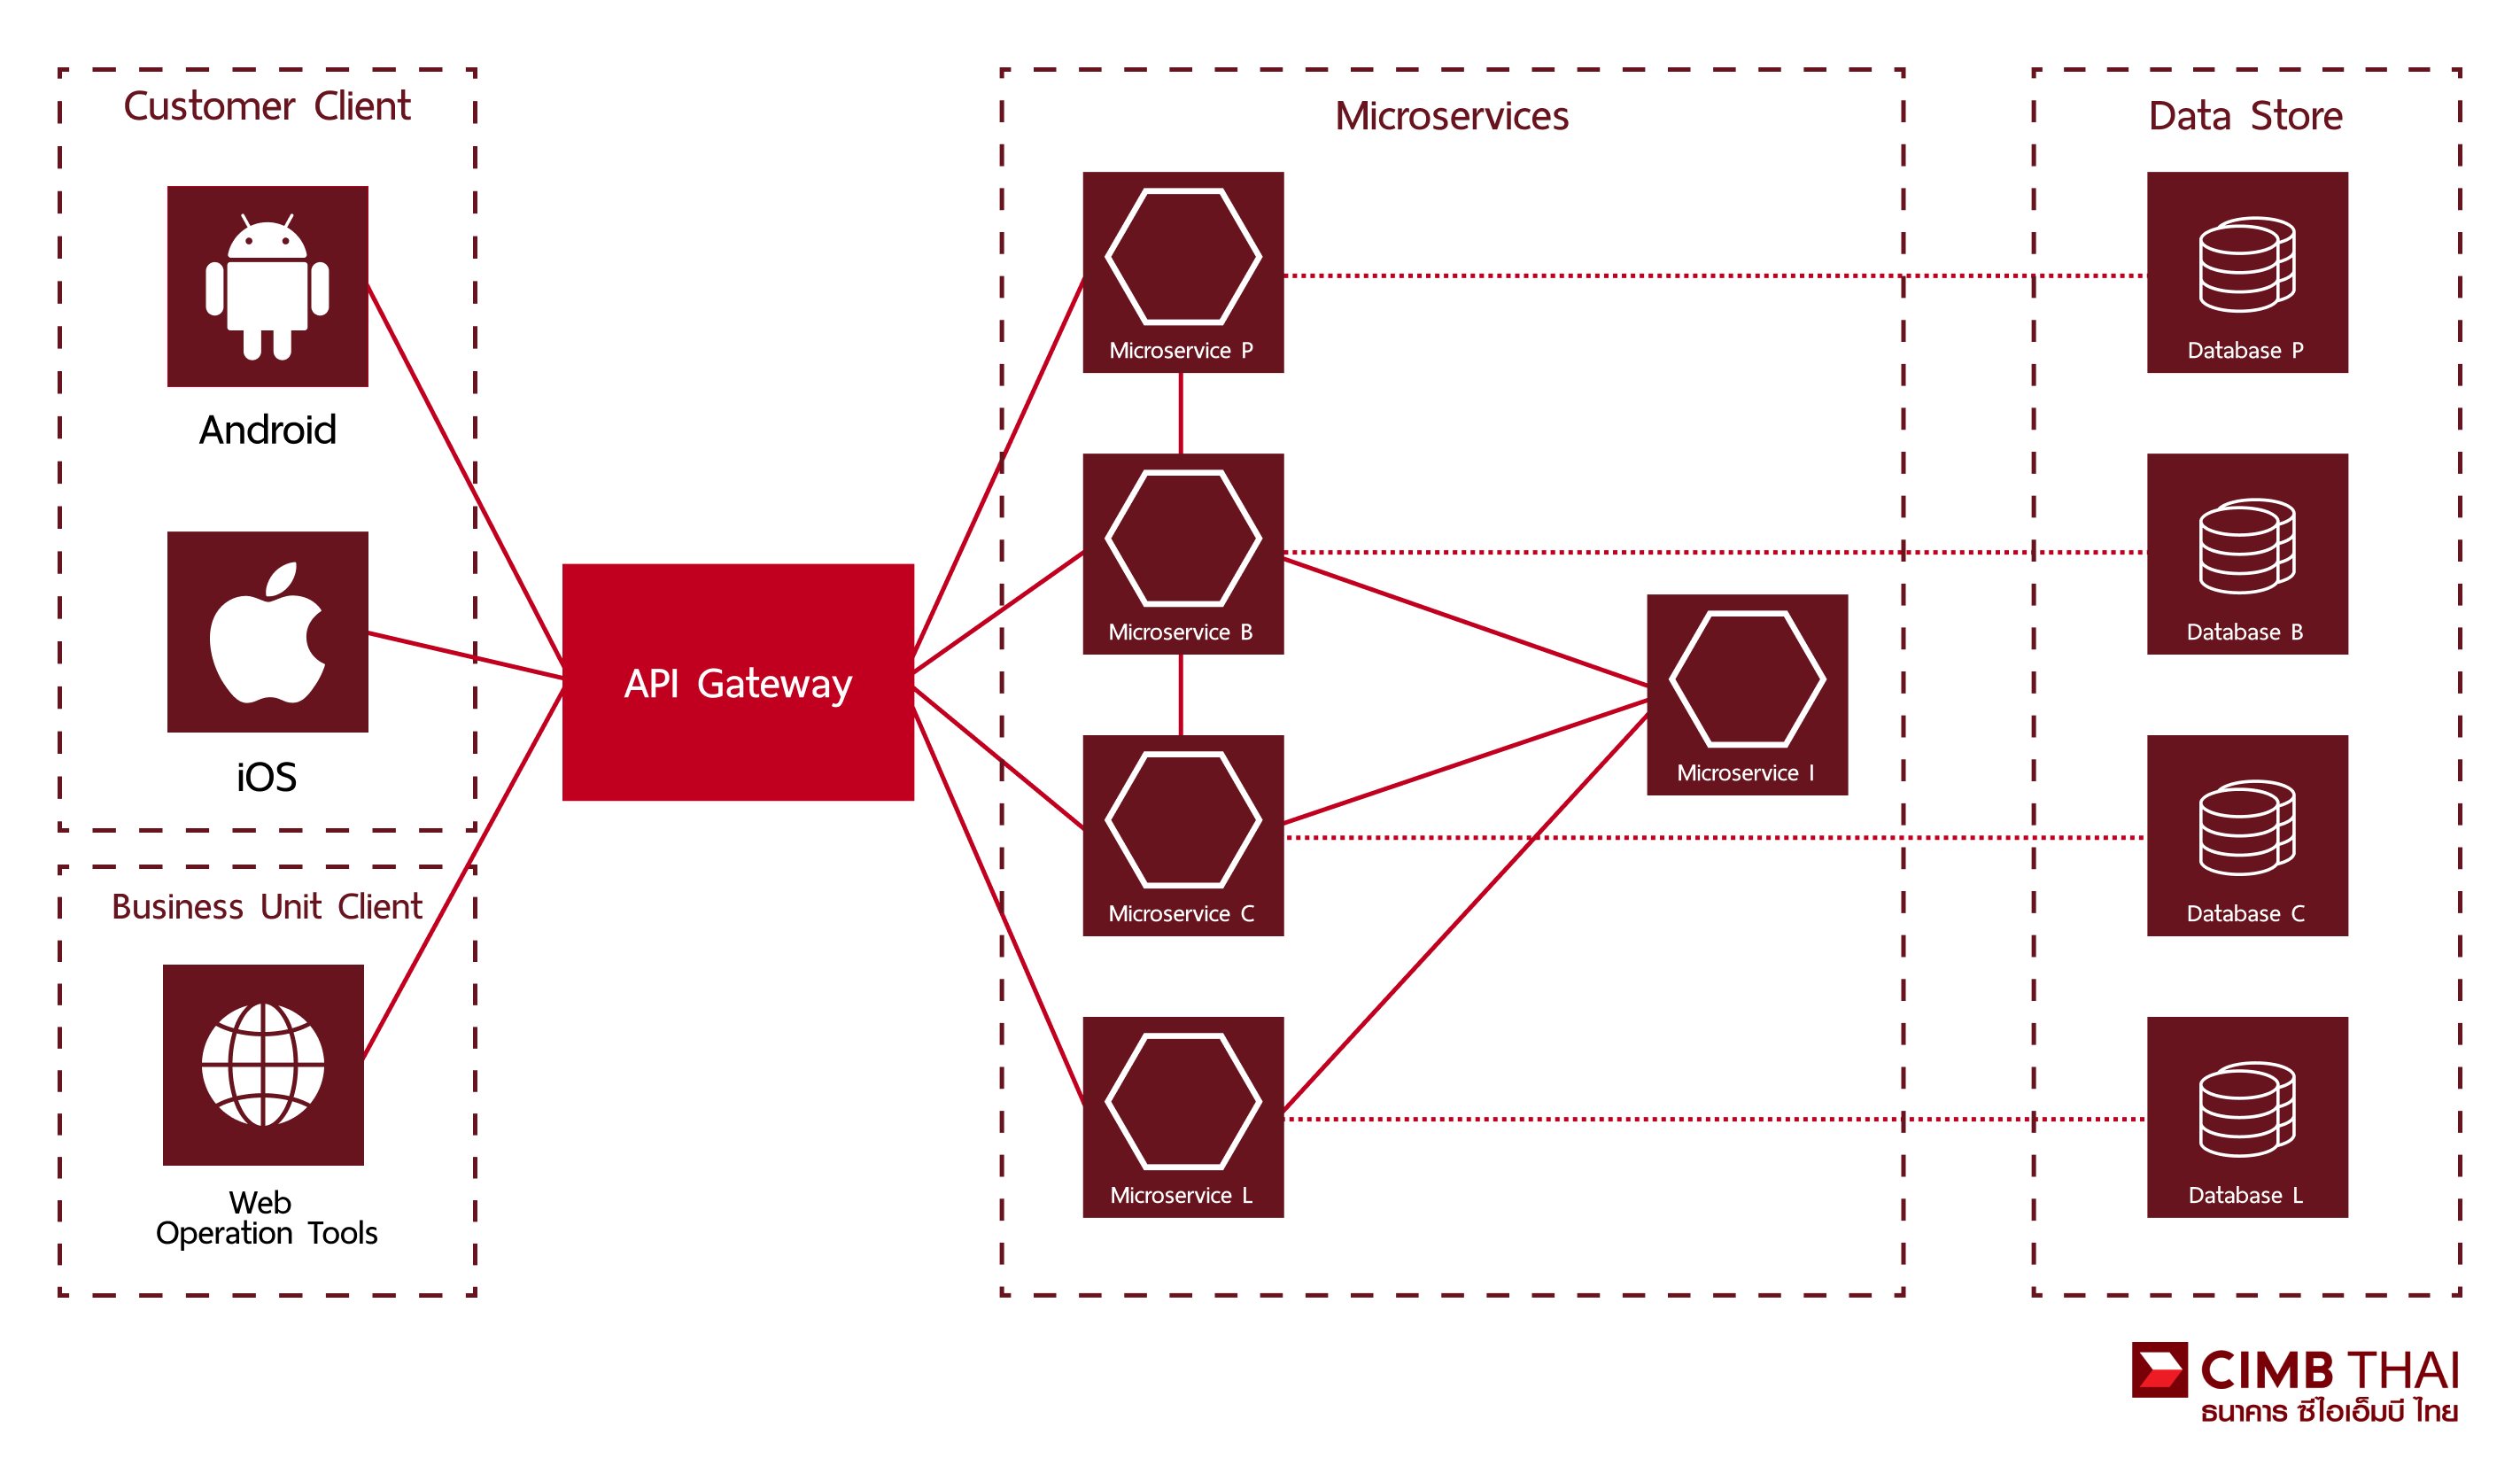
\includegraphics[width=1\textwidth]{app-structure}
%     \caption{โครงสร้างระบบการจองซื้อหุ้นกู้ในแอปพลิเคชัน ซีไอเอ็มบีไทยดิจิตอลแบงก์กิ้ง}\label{app-structure}
% \end{figure}


% \section{คุณสมบัติหลัก}
% เมื่อได้รับความต้องการจากหน่วยธุรกิจมาแล้ว ทางทีมพัฒนาจึงได้เริ่มวางแผนในส่วนต่าง ๆ ที่ต้องมีในระบบดังนี้
% \begin{enumerate}
%     \item \textbf{Term and Conditions}\newline เมื่อลูกค้าในแอปพลิเคชันและเข้ามาในส่วนการจองซื้อหุ้นเป็นครั้งแรก ลูกค้าต้องสามารถกดยอมรับข้อกำหนดการใช้งาน(Term And Conditions)ได้
%     \item \textbf{Bond Home Screen}\newline โดยลูกค้าเข้ามายังส่วนการจองซื้อหุ้นกู้แล้วสามารถเลือกได้ระหว่างจองซื้อหุ้นกู้กับประวัติการจองซื้อหุ้นกู้
%     \item \textbf{Bond Transaction History Screen}\newline ลูกค้าสามารถดูรายการประวัติการจองซื้อหุ้นกู้ได้โดยสามารถเห็น จำนวนเงินที่จองซื้อ, วันที่ทำการจองซื้อ, ระดับความน่าเชื่อถือ, อัตราดอกเบื้ย เป็นต้น
%     \item \textbf{Bond Detail Screen}\newline ลูกค้าสามารถดูรายละเอียดทั้งหมดของหุ้นกู้ได้ และสามารถจองซื้อหุ้นกู้ได้ผ่านหน้านี้
%     \item \textbf{CSA Questionnaire Screen}\newline เมื่อลูกค้าการประเมินความเสี่ยงหมดอายุ ลูกค้าจำเป็นต้องทำแบบประเมินเพื่อที่จะได้รู้ระดับของความเสี่ยงว่ารับความเสี่ยงของหุ้นกู้ได้ระดับไหนโดยระดับมีตั้งแต่ 0 - 8
%     \item \textbf{Factsheet Screen}\newline เมื่อลูกค้าต้องการจองซื้อหุ้นกู้ลูกค้าจำเป็นต้องอ่านหนังสือสรุปข้อมูลสำคัญของหุ้นกู้ แล้วกดยอมรับเพื่อจองซื้อหุ้นกู้
%     \item \textbf{Warning List (Risk Acceptance) Screen}\newline ลูกค้าจำเป็นต้องรู้ความเสี่ยงต่าง ๆ ที่ได้รับเมื่อต้องการซื้อหุ้นกู้ ซึ่งขึ้นอยู่กับเงื่อนไขต่าง ๆ เช่น ความเสี่ยงทั่วไปเมื่อต้องการจองซื้อหุ้นกู้ ความเสี่ยงที่ระดับความเสี่ยงของลูกค้าน้อยกว่าระดับความเสี่ยงของหุ้นกู้ และในกรณีที่ลูกค้าเป็นลูกค้าเปราะบางซึ่งลูกค้าต้องกดยอมรับความเสี่ยงทั้งหมดจึงจะสามารถจองซื้อหุ้นกู้ได้
%     \item \textbf{Payment Confirmation Screen}\newline ลูกค้าสามารถเลือกบัญชีที่ใช้การหักเงินได้ สามารถใส่จำนวนเงินที่ต้องการซื้อโดยขั้นต่ำเท่ากับราคาพาร์คูณกับจำหน่วยการลงทุนขั้นต่ำ สามารถกดเพิ่มลดจำนวนเงินตามราคาทวีคูณได้ และสามารถจดบันทึกรายละเอียดการจองซื้อหุ้นกู้ได้
%     \item \textbf{Benificial Information Screen}\newline ลูกค้าสามารถเลือกได้ว่าจะรับผลประโยชน์จากหุ้นกู้ทางใดไม่ว่าจะเป็นเช็ค หรือบัญชี ซึ่งถ้าเลือกบัญชีลูกค้าสามารถเลือกได้ว่าจะรับผลประโยชน์ด้วยบัญชีใด
%     \item \textbf{Receive Bond Information Screen}\newline ลูกค้าสามารถเลือกได้ว่าจะรับเอกสารหุ้นกู้ได้ระหว่างไปรษณีย์ หรือศูนย์รับฝาก ซึ่งในกรณีไปรษณีย์ลูกค้าสามารถแก้ไขที่อยู่ได้ และสามารถแก้ไขอีเมลได้ ส่วนศูนย์รับฝากสามารถเลือกศูนย์รับฝากจากรายการได้ สามารถใส่เลขที่ศูนย์รับฝากได้ และแก้ไขที่อยู่ได้ โดยลูกค้าสามารถกดจองซื้อหุ้นกู้จากหน้านี้ได้
%     \item \textbf{Review Bond Booking detail Screen}\newline ลูกค้าสามารถเห็นรายละเอียดการจองซื้อหุ้นกู้ได้ทั้งหมดและสามารถกดยืนยันรายการสั่งซื้อจากหน้านี้ได้
%     \item \textbf{Passcode Screen}\newline เมื่อกดยืนยันรายการสั่งซื้อต้องขึ้นหน้าให้ใส่รหัสผ่านของแอปพลิเคชันด้วยเพื่อยืนยันตัวตนของลูกค้าก่อนจะหักเงินบัญชี
%     \item \textbf{Receipt Screen}\newline เมื่อทำรายการสั่งซื้อเสร็จสิ้น ลูกค้าสามารถเห็นใบเสร็จสั่งซื้อ และสามารถบันทึกรูปภาพของใบเสร็จสั่งซื้อลงอัลบั้มภาพของโทรศัพท์มือถือได้อัตโนมัติ
% \end{enumerate}

% \newpage
% \section{ขอบเขตงานที่นักศึกษารับผิดชอบ}
%     นักศึกษานั้นได้อยู่ในทีม Treasury ของแผนก Digital Banking ได้มีส่วนรวมในการพัฒนาแอปพลิเคชันในส่วนการจองซื้อหุ้นกู้บนระบบปฏิบัติการ Android รวมไปถึงพัฒนาหน้า Bond Transaction History Screen 
%     บนระบบปฏิบัติการ iOS ตลอดจนทำชุดทดสอบอัตโนมัติสำหรับส่วนติดต่อลูกค้าทั้งส่วนของ Android และ iOS เพื่อการทดสอบบน Jenkins อีกด้วย

% \section{วิธีการพัฒนาระบบ}
% \subsection{Product Backlog Grooming}
% โดยทุก ๆ วันแรกของสปริ้นท์นักพัฒนาทุกคนรวมไปถึง Product Owner และ Project Manager จะมาทำความเข้าใจใน Epic และ Issue ที่มีทั้งหมดใน Sprint
% เพื่อที่จะได้ทำตามความต้องการทางธุรกิจซึ่งได้อิงตาม Epic ที่เป็นรายละเอียดความต้องของทางหน่วยธุรกิจที่ Product Owner ได้กำหนดไว้ ซึ่ง Issue 
% เกิดขึ้นจากหัวหน้านักพัฒนาได้นำ Epic มาแยกเป็น User Story ซึ่งเป็นหนึ่งในชนิดของ Issue โดยรายละเอียดของ Epic มีดังตารางที่ \ref{tableOfTask} 
% \begin{tabularx}{\linewidth}{|c|X|c|c|c|}
% 	\caption{รายละเอียดของ Epic}\label{tableOfTask} \\
% 	\hline
%     \multicolumn{1}{|c|}{\textbf{Epic ID}}	&	\multicolumn{1}{c|}{\textbf{Epic}} &	\multicolumn{1}{c|}{\textbf{Total Issue}} &	\multicolumn{1}{c|}{\textbf{Total Story Points}}	&   \multicolumn{1}{c|}{\textbf{Sprint}} \\
% 	\hline
% 	\endfirsthead
% 	\caption* {\textbf{ตารางที่ \ref{tableOfTask} (ต่อ)} รายละเอียดของ Epic} \\
% 	\hline
% 	\multicolumn{1}{|c|}{\textbf{Epic ID}}	&	\multicolumn{1}{c|}{\textbf{Epic}} &	\multicolumn{1}{c|}{\textbf{Total Issue}} &	\multicolumn{1}{c|}{\textbf{Total Story Points}}	 &	\multicolumn{1}{c|}{\textbf{Sprint}} \\
% 	\hline
% 	\endhead
% 	\hline
% 	\endfoot
% 	DA-11724 &Treasury - Product Infomation & 26 & 16 & 20\\
% 	DA-10811 &Treasury - Customer Segment & 28 & 24 & 21\\
% 	DA-11729 &Treasury - Booking & 69 & 47 & 22 - 23\\
% 	\hline
% \end{tabularx}

% นอกเหนือจากการอธิบายรายละเอียดของ Epic และ Issue ให้เข้าใจนั้น ยังมีการประเมินค่าคะแนนของ Issue ที่นักพัฒนาทุกคนต้องร่วมกันประเมินว่าแต่ละ Issue
% มีความยากง่ายแค่ไหน ใช้เวลาในการดำเนินการเท่าไร โดยการประเมินค่าคะแนนจะใช้ลำดับฟีโบนัชชีในการประเมินเพื่อให้คะแนนมีความแตกต่างกันอย่างชัดเจน
% เมื่อ Issue นั้นไม่สามารถหาคะแนนลงได้เนื่องจากว่าอาจจะใหญ่เกินไป ทำให้หัวหน้านักพัฒนาสามารถแยก Issue ให้เล็กกว่านี้ได้อีก ซึ่งการให้คะแนนจะทำไปเรื่อย ๆ
% จนกว่าทุกคนจะให้คะแนนเท่ากัน และเข้าใจเหตุผลของการให้คะแนนโดยรายละเอียดของ Issue ของแต่ละ Epic มีรายละเอียดดังตารางที่ \ref{tableOfStoryProductInfo}, \ref{tableOfStoryCustomerSeg}, \ref{tableOfStoryBookingSP22} และ \ref{tableOfStoryBookingSP23}
% \begin{tabularx}{\linewidth}{|c|X|c|c|}
% 	\caption{รายละเอียดของ Issue ของ Treasury - Product Infomation}\label{tableOfStoryProductInfo} \\
% 	\hline
%     \multicolumn{1}{|c|}{\textbf{Issue ID}}	&	\multicolumn{1}{c|}{\textbf{Issue}} &	\multicolumn{1}{c|}{\textbf{Issue Type}}  &	\multicolumn{1}{c|}{\textbf{Story Point}} \\
% 	\hline
% 	\endfirsthead
% 	\caption* {\textbf{ตารางที่ \ref{tableOfStoryProductInfo} (ต่อ)} รายละเอียดของ Issue ของ Treasury - Product Infomation} \\
% 	\hline
% 	\multicolumn{1}{|c|}{\textbf{Issue ID}}	&	\multicolumn{1}{c|}{\textbf{Issue}} &	\multicolumn{1}{c|}{\textbf{Issue Type}}  &	\multicolumn{1}{c|}{\textbf{Story Point}} \\
% 	\hline
% 	\endhead
% 	\hline
% 	\endfoot
% 	DA-12630 &[iOS][Success] Customer can see menu 'หุ้นกู้' in mini app menu &Story &1\\
% 	DA-12640 &[iOS][Success] Customer can navigate to detail and then can back to ProductList. &Story &1\\
%     DA-12606 &[iOS][Success] Customer can see T\&C when go to bond first time &Story &2\\
%     DA-12645 &[iOS][Fail] Customer can see error dialog when has error on T\&C. &Story &1\\
%     DA-12607 &[iOS][Success] Customer can see 'รายการหุ้นกู้' (bond product list) &Story &3\\
%     DA-12609 &[iOS][Success] Customer can see empty page when bond list is empty &Story &2\\
%     DA-12608 &[iOS][Fail] Customer can see error dialog when go to product list and any error occurred &Story &1\\
%     DA-12610 &[iOS][Success] On booking history tab : Customer should see empty booking history list. &Story &1\\
%     DA-12627 &[Android][Success] Customer can see 'รายละเอียดหุ้นกู้' (bond product detail) &Story &2\\
%     DA-12629 &[Android][Success] Customer can see prospectus when click 'เอกสารสรุปข้อมูลสำคัญ' in bond detail page &Story &2\\
%     DA-12628 &[Android][Success] Customer can see factsheet when click 'หนังสือชี้ชวน' in bond detail page &Story &2\\
%     DA-12615 &[Web][Success] Admin can add bond information &Story &2\\
%     DA-12616 &[Web][Success] Admin can view bond information &Story &2\\
%     DA-12617 &[Web][Success] Admin can edit bond information &Story &2\\
%     DA-12618 &[Web][Success] Admin can delete bond information &Story &2\\
%     DA-12619 &[Web][Success] Prevent XSS &Story &1\\
%     DA-14547 &[iOS][Success] Customer can see product name on the product list and product detail &Story &1\\
%     DA-14548 &[Android][Success] Customer can see product name on the product list and product detail &Story &1\\
% 	\hline
% \end{tabularx}

% จากตารางที่ \ref{tableOfStoryProductInfo}  นี้จะเป็น Issue ทั้งหมดของ Epic Treasury - Product Info. ที่เกี่ยวกับหน้ารายการหุ้นกู้ และรายละเอียดหุ้นกู้ โดยมี Web Operation Tool เป็นตัวจัดการข้อมูลทั้งเพิ่ม
% ลบ และแก้ไข โดยสามารถกดเข้าไปดูรายละเอียดหุ้นกู้แต่ละรายการได้ ซึ่งทีม Treasury ได้รับมอบหมายให้ดูส่วนของรายละเอียดหุ้นกู้ และเว็บไซต์เพื่อจัดการข้อมูล

% \clearpage
% \begin{tabularx}{\linewidth}{|c|X|c|c|}
% 	\caption{รายละเอียดของ Issue ของ Treasury - Customer Segment}\label{tableOfStoryCustomerSeg} \\
% 	\hline
%     \multicolumn{1}{|c|}{\textbf{Issue ID}}	&	\multicolumn{1}{c|}{\textbf{Issue}} &	\multicolumn{1}{c|}{\textbf{Issue Type}}  &	\multicolumn{1}{c|}{\textbf{Story Point}} \\
% 	\hline
% 	\endfirsthead
% 	\caption* {\textbf{ตารางที่ \ref{tableOfStoryCustomerSeg} (ต่อ)} รายละเอียดของ Issue ของ Treasury - Customer Segment} \\
% 	\hline
% 	\multicolumn{1}{|c|}{\textbf{Issue ID}}	&	\multicolumn{1}{c|}{\textbf{Issue}} &	\multicolumn{1}{c|}{\textbf{Issue Type}}  &	\multicolumn{1}{c|}{\textbf{Story Point}} \\
% 	\hline
% 	\endhead
% 	\hline
% 	\endfoot
% 	DA-13567 &[API] Migrate factsheet url from bond information to legal-document. &Story &2\\
% 	DA-13388 &[iOS][Success] Customer can see factsheet when bond type is PO and customer type is PO &Story &1\\
%     DA-13388 &[iOS][Success] Customer can see factsheet when bond type is PO and customer type is HNW &Story &1\\
%     DA-13389 &[iOS][Success] Customer can see factsheet when bond type is PO and customer type is UHNW &Story &1\\
%     DA-13414 &[Android][Success] Customer can see factsheet when bond type is PO and customer type is PO &Story &1\\
%     DA-13415 &[Android][Success] Customer can see factsheet when bond type is PO and customer type is HNW &Story &1\\
%     DA-13416 &[Android][Success] Customer can see factsheet when bond type is PO and customer type is UHNW &Story &1\\
%     DA-13399 &[iOS][Success] Customer can see eligible list &Story &2\\
%     DA-13425 &[Android][Success] Customer can see eligible list &Story &2\\
%     DA-13400 &[iOS][Success] Customer can accept eligible. &Story &1\\
%     DA-13426 &[Android][Success] Customer can accept eligible. &Story &1\\
%     DA-13401 &[iOS][Success] Customer can see eligible detail &Story &1\\
%     DA-13427 &[Android][Success] Customer can see eligible detail&Story &1\\
%     DA-13438 &[WebOperation][Success] PO can create questionnaire for self declare. &Story &1\\
%     DA-13533 &[Web][Success] [API] Return data from ivp &Story &1\\
%     DA-13432 &[Android][Fail] Customer can see error dialog when can't get eligible legal document &Story &1\\
%     DA-13406 &[iOS][Fail] Customer can see error dialog when can't get eligible legal document &Story &1\\
%     DA-13407 &[iOS][Fail] Customer can see error dialog when can't accept eligible legal document &Story &1\\
%     DA-13433 &[Android][Fail] Customer can see error dialog when can't accept eligible legal document &Story &1\\
%     DA-13402 &[iOS][Fail] Customer can see error dialog when can't get factsheet legal document &Story &1\\
%     DA-13428 &[Android][Fail] Customer can see error dialog when can't get factsheet legal document &Story &1\\
%     DA-13403 &[iOS][Fail] Customer can see error dialog when can't accept factsheet legal document &Story &1\\
%     DA-13429 &[Android][Fail] Customer can see error dialog when can't accept factsheet legal document &Story &1\\
%     DA-14204 &[Backend] Prepare api booking primary bond. &Task &2\\
% 	\hline
% \end{tabularx}

% จากตารางที่ \ref{tableOfStoryCustomerSeg}  นี้จะเป็น Issue ทั้งหมดของ Epic Treasury - Customer Segment ที่เกี่ยวกับส่วนของการส่วนการยืนยันตัวตนเพื่อระบุลูกค้าว่าเป็นประเภทใด ได้แก่ ผู้ลงทุนรายใหญ่, ผู้ลงทุนรายใหญ่ และผู้ลงทุนรายใหญ่พิเศษ
% เมื่อลูกค้ายืนยันตัวตนสำเร็จแล้วลูกค้าจะต้องอ่านเอกสารสรุปข้อมูลสำคัญของหุ้นกู้แล้วยอมรับ เมื่อลูกค้ายืนยันเอกสารสรุปข้อมูลสำคัญหุ้นกู้แล้ว ลูกค้าต้องยอมรับความเสี่ยงของการจองซื้อหุ้นกู้ได้
% โดยทีม Treasury ได้รับผิดชอบในส่วนของเอกสารสรุปข้อมูลสำคัญ และการยอมรับรายการความเสี่ยงของลูกค้า


% \begin{tabularx}{\linewidth}{|c|X|c|c|}
% 	\caption{รายละเอียดของ Issue ของ Treasury - Booking (Sprint 22)}\label{tableOfStoryBookingSP22} \\
% 	\hline
%     \multicolumn{1}{|c|}{\textbf{Issue ID}}	&	\multicolumn{1}{c|}{\textbf{Issue}} &	\multicolumn{1}{c|}{\textbf{Issue Type}}  &	\multicolumn{1}{c|}{\textbf{Story Point}} \\
% 	\hline
% 	\endfirsthead
% 	\caption* {\textbf{ตารางที่ \ref{tableOfStoryBookingSP22} (ต่อ)} รายละเอียดของ Issue ของ Treasury - Booking (Sprint 22)} \\
% 	\hline
% 	\multicolumn{1}{|c|}{\textbf{Issue ID}}	&	\multicolumn{1}{c|}{\textbf{Issue}} &	\multicolumn{1}{c|}{\textbf{Issue Type}}  &	\multicolumn{1}{c|}{\textbf{Story Point}} \\
% 	\hline
% 	\endhead
% 	\hline
% 	\endfoot
% 	DA-14907 &[iOS][Success] Customer can see bond detail and check see suitability (CSA) expired &Story &1\\
% 	DA-14910 &[Android][Success] Customer can see bond detail and check see suitability (CSA) expired &Story &1\\
%     DA-14912 &[iOS][Fail] Customer can see bond detail and check see suitability (CSA) expired when get customer profile risk service not available &Story &1\\
%     DA-14911 &[Android][Fail] Customer can see bond detail and check see suitability (CSA) expired when get customer profile risk service not available. &Story &1\\
%     DA-14529 &[iOS][Success] Customer can see suitability test expired (CSA). &Story &1\\
%     DA-14809 &[Android][Success] Customer can see suitability test expired (CSA). &Story &1\\
%     DA-14530 &[iOS][Success] Customer can see and accept T\&C for suitability test (CSA). &Story &1\\
%     DA-14810 &[Android][Success] Customer can see and accept T\&C for suitability test (CSA). &Story &1\\
%     DA-14531 &[iOS][Fail] Customer can see error dialog when get T\&C not available. &Story &1\\
%     DA-14811 &[Android][Fail] Customer can see error dialog when get T\&C not available. &Story &1\\
%     DA-14533 &[iOS][Fail] Customer can see error dialog when accept T\&C not available. &Story &1\\
%     DA-14820 &[Android][Fail] Customer can see error dialog when accept T\&C not available. &Story &1\\
%     DA-14534 &[iOS][Success]Customer can see suitability test (CSA). &Story &3\\
%     DA-14821 &[Android][Success]Customer can see suitability test (CSA). &Story &3\\
%     DA-14535 &[iOS][Success] Customer can see and accept result suitability test (CSA). &Story &2\\
%     DA-14822 &[Android][Success] Customer can see and accept result suitability test (CSA). &Story &2\\
%     DA-14536 &[iOS][Fail] Customer can see error dialog when get result suitability from legal-doc not available. &Story &1\\
%     DA-14823 &[Android][Fail] Customer can see error dialog when get result suitability from legal-doc not available. &Story &1\\
%     DA-14684 &[iOS][Fail] Customer can see error dialog when accept result suitability from legal-doc not available. &Story &1\\
%     DA-14840 &[Android][Fail] Customer can see error dialog when accept result suitability from legal-doc not available. &Story &1\\
%     DA-14807 &[Backend] Create order bond. &Story &5\\
%     DA-14527 &[iOS][Success] Customer can see review order page. &Story &3\\
%     DA-14790 &[Android][Success] Customer can see review order page. &Story &3\\
%     DA-14792 &[Android][Fail] Customer can see error dialog when create order not available. &Story &1\\
%     DA-14681 &[iOS][Success] Customer can see booking history &Story &2\\
%     DA-14871 &[Android][Success] Customer can see booking history &Story &2\\
%     DA-14528 &[iOS][Fail] Customer can see error dialog when create order not available. &Story &1\\
%     DA-14682 &[iOS][Fail] Customer see error when cannot get booking history &Story &1\\
%     DA-14873 &[Android][Fail] Customer see error when cannot get booking history &Story &1\\
%     DA-15333 &[Android][Success] Initial Mini app payment processor &Task &1\\
%     DA-15332 &[iOS][Success] Initial Mini app payment processor &Task &1\\
%     DA-15536 &[iOS][Success] Customer can see passcode for confirm booking bond &Story &1\\
%     DA-15560 &[iOS][Fail] Customer can't booking bond when customer never have customer type. &Story &0\\
% 	\hline
% \end{tabularx}

% จากตารางที่ \ref{tableOfStoryBookingSP22}  นี้จะเป็น Issue ของ Treasury - Booking ที่เกี่ยวกับส่วนของการจองซื้อหุ้นกู้โดยจะประกอบไปด้วยสองส่วนหลัก ๆ คือ ส่วนการจองซื้อ 
% และแบบประเมินความเสี่ยงของผู้ลงทุน ซึ่งทีม Treasury ได้รับผิดชอบในส่วนแบบประเมินความเสี่ยงของผู้ลงทุน และการสร้างคำสั่งซื้อ โดยลูกค้าจะทำแบบประเมินความเสี่ยงของผู้ลงทุนเมื่ออายุการประเมินความเสี่ยงของลูกค้าหมดอายุ

% \begin{tabularx}{\linewidth}{|c|X|c|c|}
% 	\caption{รายละเอียดของ Issue ของ Treasury - Booking (Sprint 23)}\label{tableOfStoryBookingSP23} \\
% 	\hline
%     \multicolumn{1}{|c|}{\textbf{Issue ID}}	&	\multicolumn{1}{c|}{\textbf{Issue}} &	\multicolumn{1}{c|}{\textbf{Issue Type}}  &	\multicolumn{1}{c|}{\textbf{Story Point}} \\
% 	\hline
% 	\endfirsthead
% 	\caption* {\textbf{ตารางที่ \ref{tableOfStoryBookingSP23} (ต่อ)} รายละเอียดของ Issue ของ Treasury - Booking (Sprint 23)} \\
% 	\hline
% 	\multicolumn{1}{|c|}{\textbf{Issue ID}}	&	\multicolumn{1}{c|}{\textbf{Issue}} &	\multicolumn{1}{c|}{\textbf{Issue Type}}  &	\multicolumn{1}{c|}{\textbf{Story Point}} \\
% 	\hline
% 	\endhead
% 	\hline
% 	\endfoot
% 	DA-15530 &[iOS][Fail] Customer input passcode wrong. &Story &1\\
% 	DA-15558 &[iOS][Fail] Customer can't confirm booking bond when insufficient amount&Story &1\\
%     DA-15552 &[iOS][Fail] Customer input passcode exceed pin attempt.&Story &2\\
%     DA-15541 &[iOS][Fail] Customer can't confirm booking bond when transaction limit.&Story &1\\
%     DA-15557 &[iOS][Fail][Confirm Step] Customer can't confirm booking bond when exceed quota limit. &Story &1\\
%     DA-15555 &[iOS][Fail] Customer input passcode and show error dialog when service not available &Story &1\\
%     DA-15531 &[iOS][Success] Customer can see slip after confirm booking bond &Story &3\\
%     DA-15533 &[iOS][Success] Save slip image after comfirm booking's bond is success &Story &1\\
%     DA-15534 &[iOS][Fail] Customer can't allow permission when save slip. &Story &1\\
%     DA-15535 &[Web Operation] Admin can see transaction history. &Story &1\\
%     DA-15693 &[iOS][Success] Customer can booking bond when Customer type match Product Type. &Story &2\\
%     DA-15537 &[iOS][Fail] Customer can't booking bond when Customer type lower than Product Type. &Story &1\\
%     DA-15556 &[API] Handle error create booking &Story &2\\
%     DA-15559 &[API] Handle error confirm booking. &Story &2\\
% 	\hline
% \end{tabularx}

% จากตารางที่ \ref{tableOfStoryBookingSP23}  นี้จะเป็น Issue ของ Treasury - Booking ที่เกี่ยวกับส่วนของการยืนยันคำสั่งซืิ้อหุ้นกู้ และการแจ้งเตือนผ่านอีเมล 
% โดยการยืนยันคำสั่งซื้อหุ้นกู้นั้นจะต้องมีการใส่รหัสผ่านที่ลูกค้าได้ตั้งไว้เพื่อระบุตัวตนว่าคือลูกค้าคนนั้นจริง ๆ และเมื่อยืนยันคำสั่งซื้อลูกค้าจะต้องเห็นหน้าใบเสร็จ 
% และสามารถบันทึกรูปภาพของใบเสร็จสั่งซื้อลงอัลบั้มภาพของโทรศัพท์มือถือได้อัตโนมัติ

% โดยที่ Issue แต่ละอันนั้นจะมี Acceptance Criteria ที่แตกต่างกันตามที่หัวหน้านักพัฒนาได้คุยกับ Product Owner ไว้แต่ละ Issue มีเป้าหมายอะไร
% และแต่ละทีมนั้นจะมีนิยามของคำเสร็จที่แตกต่างกันโดยที่ทีม Treasury นั้นมีนิยามว่านักพัฒนาทุกคนไม่ว่าจะพัฒนาในส่วนไหนต้องสร้างชุดทดสอบให้สำเร็จด้วย
% ตามส่วนที่ตนเองนั้นได้พัฒนาถ้าเป็นในส่วนของ Mobile Application ต้องทำ UI automated test ให้สำเร็จ และถ้าพัฒนาฝั่ง API ต้องทำ Unit test
% ให้เสร็จสิ้น

% \subsection{Sprint Planning}
% ในส่วนนี้จะเป็นส่วนที่นักพัฒนาทุกคนต้องมาช่วยกันวางแผน และสร้าง Sequence Diagram เพื่อที่ฝั่ง Frontend และ Backend
% จะได้ทำความเข้าใจว่าจะเกิดอะไรขึ้นบ้างเมื่อแอปพลิเคชันอยู่ในหน้าต่างนั้น ๆ โดยที่จะพูดถึงเรื่องการร้องขอข้อมูลจาก Frontend
% ไปยัง Backend หรือ Backend ร้องขอข้อมูลกันเองโดยทางทีม Treasury แบ่งได้เป็น 2 ส่วนหลักคือ

% \setcounter{secnumdepth}{5} 
% \subsubsection{Management Part}
% ส่วน Management จะเป็นส่วนจัดการข้อมูลของหุ้นกู้ทั้งหมดไม่ว่าจะเป็นการเพิ่ม ลบ และแก้ไขโดยมี Sequence Diagram ดังนี้

% \paragraph{เพิ่มข้อมูลหุ้นกู้}
% \begin{figure}[H]
%     \centering
%     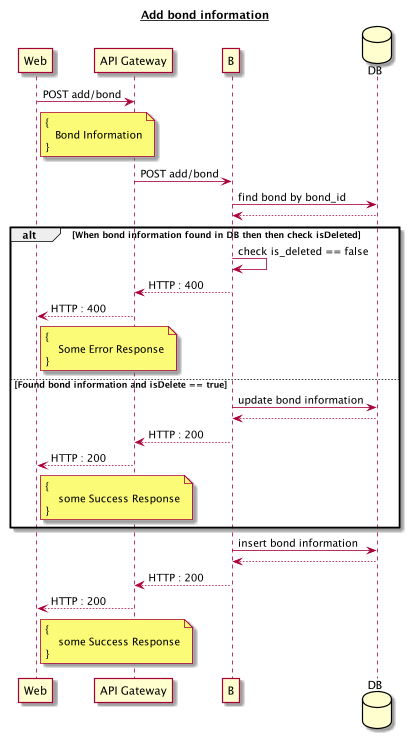
\includegraphics[width=0.5\textwidth]{bond-information-add}
%     \caption{Sequence Diagram ของขั้นตอนการเพิ่มข้อมูลหุ้นกู้}\label{bond-information-add}
% \end{figure}
% การทำงานคือเมื่อ Web Operation Tools เพิ่มหุ้นกู้เข้าไปยัง Backend จะมีการตรวจสอบก่อนว่าหุ้นกู้นั้นมีอยู่ในระบบหรือยัง
% ถ้ามีแล้วจะไปตรวจสอบ Flag ที่สร้างไว้ตัวหนึ่งว่าหุ้นกู้นั้นมีสถานะถูกลบหรือเปล่า ถ้าถูกลบจะอัพเดทหุ้นตัวเดิมแล้วเปลี่ยนสถานะเป็นไม่ถูกลบ
% แต่ถ้ายังไม่ถูกลบจะเพิ่มล้มเหลว และถ้ายังไม่มีหุ้นกู้ก็จะสามารถเพิ่มเข้าไปในระบบได้ทันที

% \paragraph{แก้ไขข้อมูลหุ้นกู้}
% \begin{figure}[H]
%     \centering
%     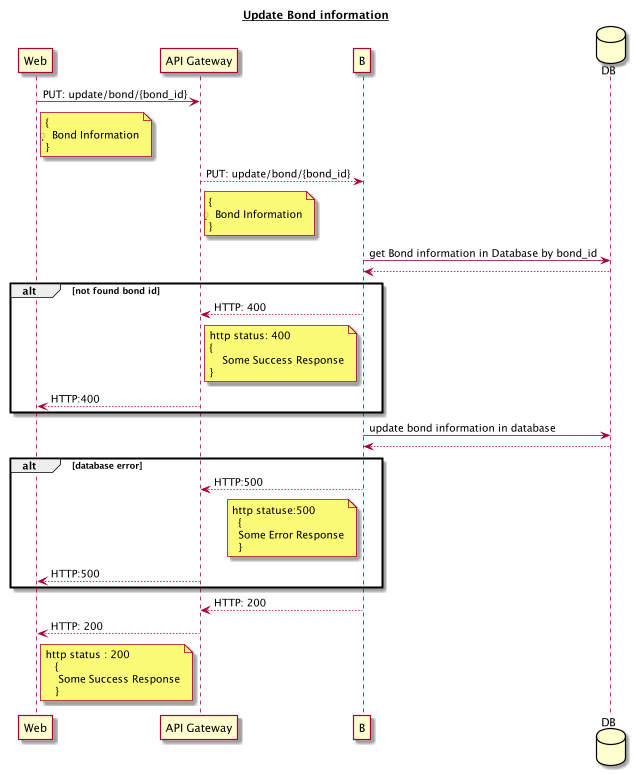
\includegraphics[width=0.5\textwidth]{bond-information-update}
%     \caption{Sequence Diagram ของขั้นตอนการแก้ไขข้อมูลหุ้นกู้}\label{bond-information-update}
% \end{figure}
% การทำงานคือเมื่อ Web Operation Tools ต้องการแก้ไขข้อมูลขั้นตอนแรกต้องมีการตรวจสอบก่อนว่าหุ้นกู้นี้มีอยู่จริงหรือเปล่า
% ถ้ามีอยู่ก็สามารถแก้ไขได้ตามปกติ แต่ถ้าไม่มีก็จะทำการแก้ไขล้มเหลว

% \paragraph{ลบข้อมูลหุ้นกู้}
% \begin{figure}[H]
%     \centering
%     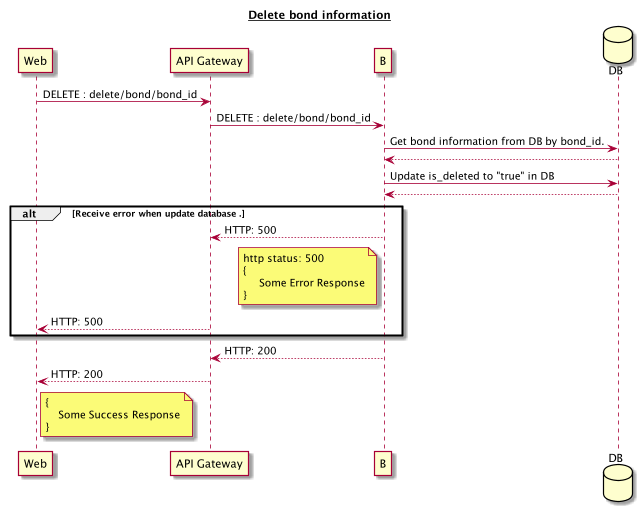
\includegraphics[width=0.5\textwidth]{bond-information-delete}
%     \caption{Sequence Diagram ของขั้นตอนการลบข้อมูลหุ้นกู้}\label{bond-information-delete}
% \end{figure}
% การทำงานคือเมื่อ Web Operation Tools เต้องการลบข้อมูลขั้นตอนแรกต้องมีการตรวจสอบก่อนว่าหุ้นกู้นี้มีอยู่จริงหรือเปล่า
% ถ้ามีอยู่ก็สามารถลบได้ตามปกติ แต่ถ้าไม่มีก็จะทำการลบล้มเหลว

% \paragraph{เรียกข้อมูลหุ้นกู้}
% \begin{figure}[H]
%     \centering
%     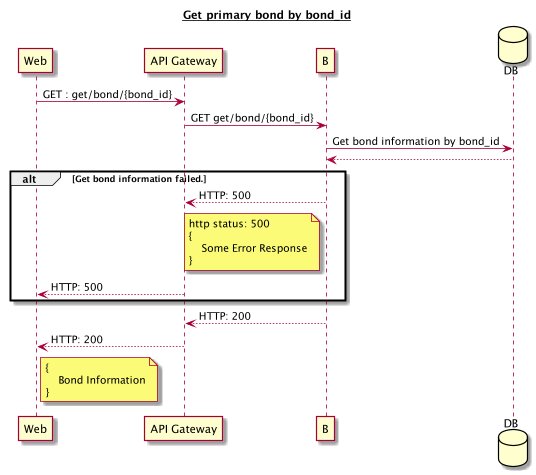
\includegraphics[width=0.5\textwidth]{bond-information-get}
%     \caption{Sequence Diagram ของขั้นตอนการเรียกข้อมูลหุ้นกู้}\label{bond-information-get}
% \end{figure}
% การทำงานคือเมื่อ Web Operation Tools ต้องการเรียกดูข้อมูลขั้นตอนแรกต้องมีการตรวจสอบก่อนว่าหุ้นกู้นี้มีอยู่จริงหรือเปล่า
% ถ้ามีอยู่ก็สามารถเรียกดูได้ตามปกติ แต่ถ้าไม่มีก็จะทำการเรียกดูล้มเหลว

% \newpage
% \subsubsection{Main Part}
% โดยในส่วนนี้เป็นส่วนหลักในการจองซื้อหุ้นกู้ซึ่งแบ่งออกได้ดังนี้

% \paragraph{สร้างคำสั่งการจองซื้อหุ้นกู้}
% \begin{figure}[H]
%     \centering
%     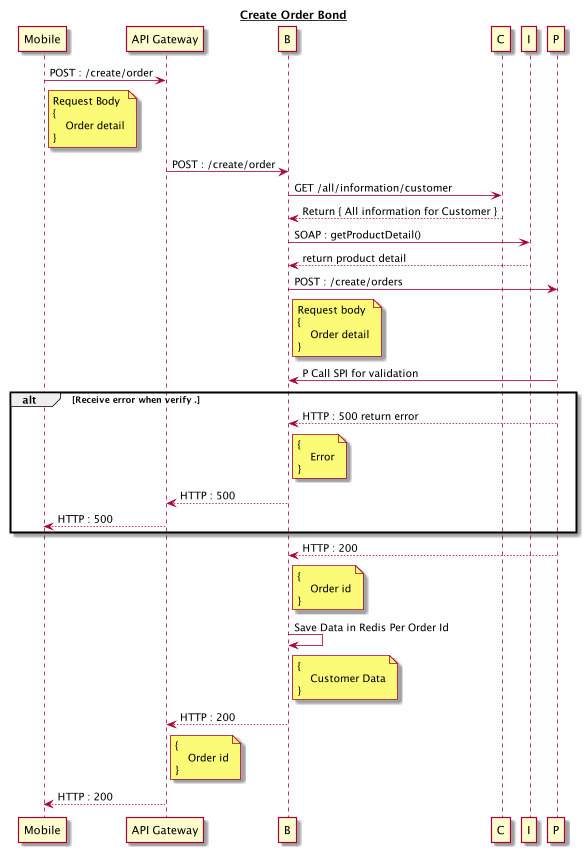
\includegraphics[width=0.5\textwidth]{booking-create-order}
%     \caption{Sequence Diagram ของขั้นตอนสร้างคำสั่งการจองซื้อหุ้นกู้}\label{booking-create-order}
% \end{figure}
% การสร้างคำสั่งการจองซื้อนั้นเป็นขั้นตอนที่มี Logic มากมายที่ใช้เพราะว่าการที่จะสร้างคำสั่งการจองซื้อได้ต้องผ่านส่วนต่าง ๆ ของแอปพลิเคชันมาทั้งหมดตามที่กำหนดไว้
% จึงต้องตรวจสอบสถานะในการผ่านหน้าต่าง ๆ มา อีกทั้งยังมีการตรวจสอบข้อมูลทั้งหมดของลูกค้าว่าใช่ลูกค้าจริง ๆ หรือเปล่าที่เป็นผู้กดจองซื่้อ และสุดท้ายก็ตรวจสอบ
% ว่าหุ้นกู้ยังสามารถจองซื้อได้อยู่หรือไม่

% \paragraph{ยืนยันการจองซื้อหุ้นกู้}
% \begin{figure}[H]
%     \centering
%     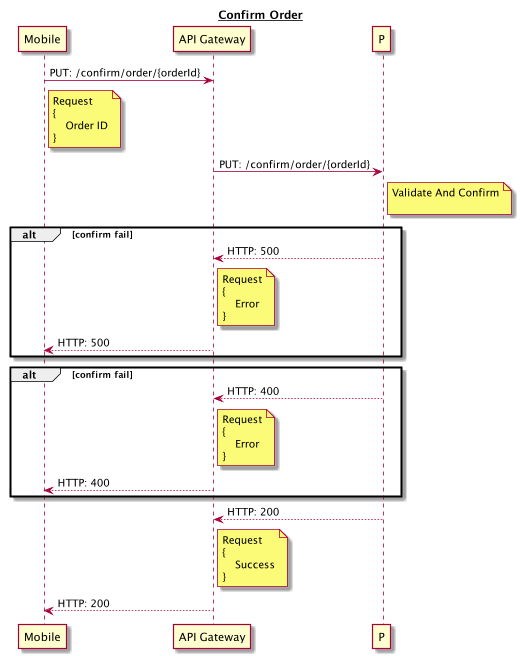
\includegraphics[width=0.5\textwidth]{booking-confirm-order}
%     \caption{Sequence Diagram ของขั้นตอนยืนยันการจองซื้อหุ้นกู้}\label{booking-confirm-order}
% \end{figure}
% ในขั้นตอนนี้ก่อนที่จะมีการยืนยันได้นั้นต้องผ่านการสร้างคำสั่งการจองซื้อมาก่อนจึงจะสามารถกดยืนยันได้ และจะมีการตรวจสอบยอดเงินคงเหลือในบัญชี
% จำนวนหุ้นกู้ที่สามารถซื้อได้ต่อวัน และ จำนวนหุ้นกู้ที่เหลือเพียงพอต่อการจองซื้อหุ้นกู้หรือไม่

% \subsection{Develop And Test}
% เป็นช่วงที่นักพัฒนาทุกคนจะพัฒนาในส่วนต่าง ๆ ในแอปพลิเคชันตาม Issue ใน Scrum Active Sprint Board ดังรูปที่ \ref{scrum-active-sprint-board} 
% \begin{figure}[H]
%     \centering
%     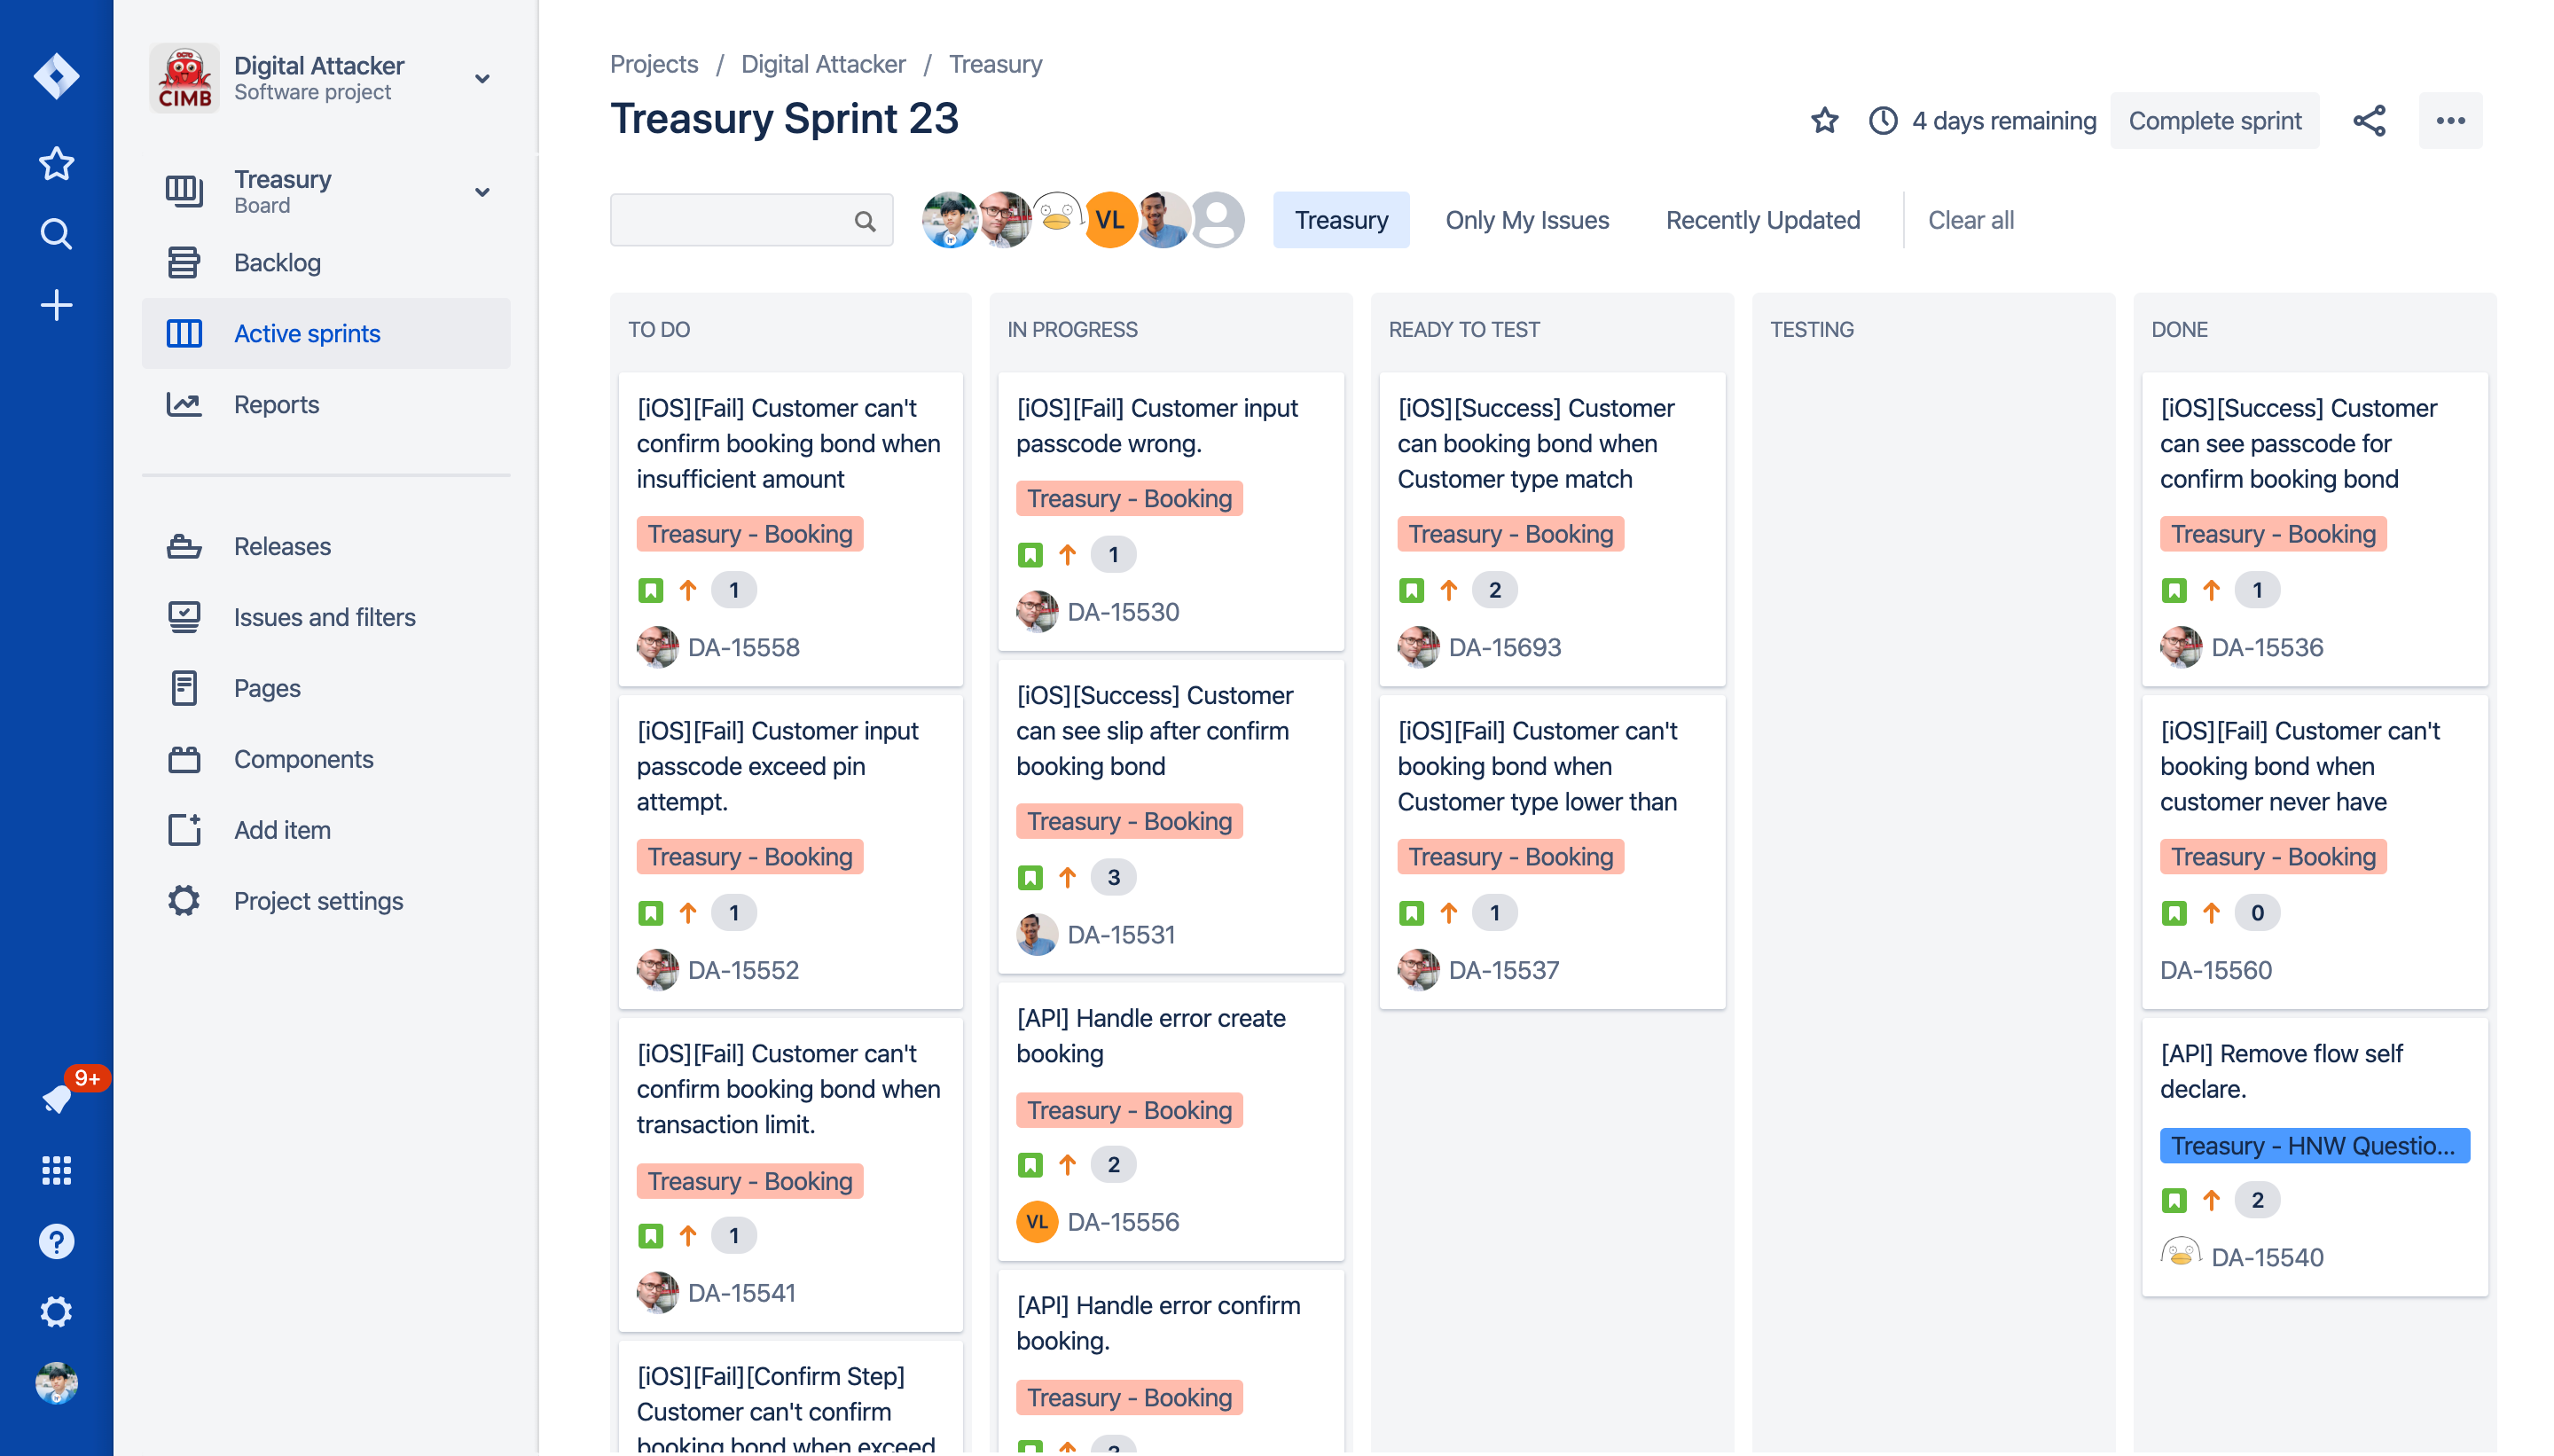
\includegraphics[width=1\textwidth]{scrum-active-sprint-board}
%     \caption{หน้าการใช้งาน Scrum Active Sprint Board}\label{scrum-active-sprint-board}
% \end{figure}
% โดยจะมีสถานะต่าง ๆ ของ Issue ดังนี้
% \subsubsection{To Do}
% สถานะนี้เป็น Issue ที่มาจาก Product Backlog เป็น Issue ทั้งหมดที่ต้องทำให้เสร็จภายใน Sprint นี้
% \subsubsection{In Progress}
% สถานะนี้เป็นสถานะที่ Issue กำลังถูกทำอยู่โดยถูกมอบหมายให้กับนักพัฒนาแต่ละคนรับผิดชอบ ซึ่งนักพัฒนาหนึ่งคนสามารถถือ Issue ได้เพียงแค่คนละ 1 Issue เพราะว่า
% ในกรณีที่นักพัฒนาถือ Issue ไว้พร้อมกัน 2 Issue แล้วนักพัฒนาทำอีกส่วนหนึ่งยังไม่เสร็จจะเป็นการ Block การทำงานของพัฒนาคนอื่นให้ช้ากว่าเดิม
% \subsubsection{Ready To Test}
% สถานะนี้เป็นสถานะที่ Issue ถูกพัฒนาเสร็จแล้วตาม Acceptance Criteria และส่งมอบต่อให้ Quality Assurance เพื่อทดสอบตาม Acceptance Criteria ที่ถูกตั้งไว้
% \subsubsection{Testing}
% สถานะนี้เป็นสถานะที่ Issue ถูกทดสอบโดย Quality Assurance หากมีกรณีไหนที่นักพัฒนาทำไม่ถูกต้องตาม Acceptance Criteria จะถูก Quality Assurance ลากไป Issue กลับไปยัง To Do เพื่อให้นักพัฒนาแก้ไข้ให้ถูกต้อง
% \subsubsection{Done}
% สถานะนี้เป็นสถานะที่ Issue ถูกพัฒนาเสร็จสิ้น ถูกต้องตาม Acceptance Criteria ทั้งหมด และเสร็จตามทั้งหมดตามนิยามของคำว่าเสร็จของทีมซึ่งคือการที่นักพัฒนาทุกคนต้องเขียนชุดทดสอบในส่วนที่ตนเองนั้นได้พัฒนาให้เสร็จสิ้น

% จากข้างต้นที่ว่าแต่ละ Issue นั้นจะ Acceptance Criteria ที่แตกต่างกันไปตามที่ Product Owner ได้กำหนดไว้ซึ่งจะมีการเขียนรายละเอียดเอาไว้ในคำอธิบายของ Issue ดังตัวอย่างจากรูปที่ \ref{acceptance-criteria}
% \begin{figure}[H]
%     \centering
%     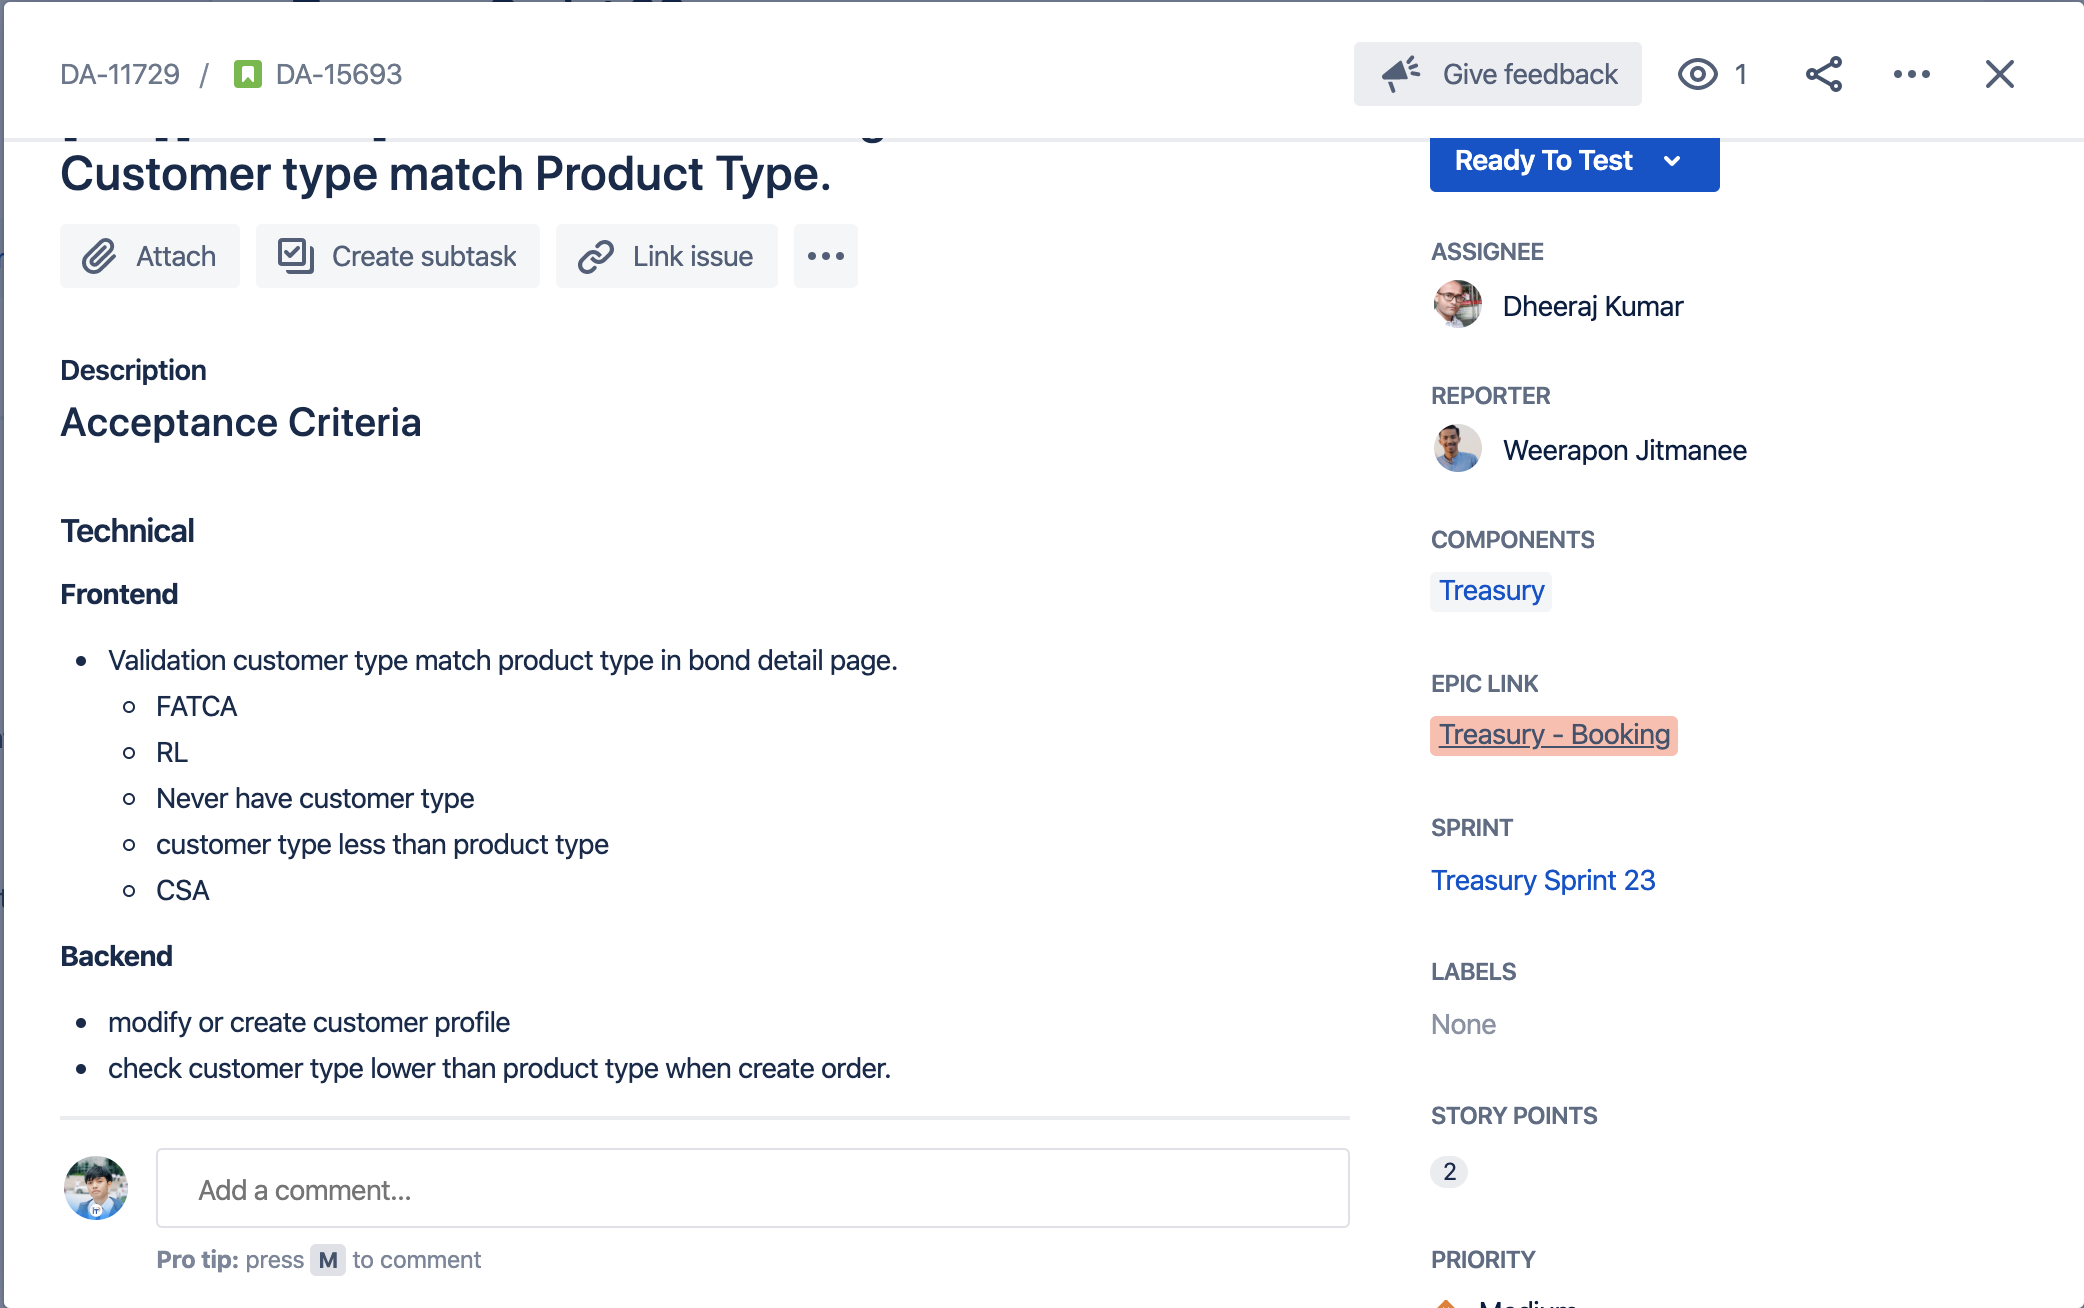
\includegraphics[width=1\textwidth]{acceptance-criteria}
%     \caption{ตัวอย่างของการกำหนด Acceptance Criteria}\label{acceptance-criteria}
% \end{figure}

% หลังจากที่นักพัฒนาได้พัฒนา Issue ที่ตนเองได้รับผิดชอบเสร็จสิ้นแล้วในสถานนะของ Ready to Test นักพัฒนาต้องทำการ Push โค้ดส่วนที่พัฒนาเสร็จขึ้นไปยัง Git 
% เพื่อที่จะให้ Jenkins ที่เป็น CI/CD ของ Digital Banking นั้น Build ส่วนพัฒนาให้อยู่ในรูปของ Dependencies ที่ Super App สามารถเรียกไปใช้งานได้
% เพื่อที่จะได้ให้ Quality Assurance ได้ทดสอบในสภาพแวดล้อมของ SIT

% \subsection{Daily Stand-up}
% เป็นกิจกรรมที่จะมีการมาอัพเดทงานและปัญหาที่เจอในวันก่อน ๆ และบอกสิ่งที่จะทำในวันนี้ซึ่งจะทำในทุก ๆ เช้าของวันทำงานโดยถ้ามีปัญหาเกิดขึ้น
% ทีมจะช่วยกันหาทางแก้ปัญหาเพื่อให้นักพัฒนาคนนั้นสามารถทำงานต่อได้ เช่น 
% เมื่อเกิดปัญหาที่นักพัฒนาคนนั้นมีส่วนที่ต้องรอทีมอื่นแก้ไขในส่วนที่ทีมอื่นทำผิดพลาดอยู่ ทำให้นักพัฒนาในทีมไม่สามารถทำงานได้เพราะต้องรอส่วนที่ผิดพลาดนั้นอยู่
% ซึ่งในกรณีนี้ทุกคนในทีมก็จะหาทางมาแก้ไขปัญหาให้ได้ เพื่อที่งานในแต่ละวันนั้นจะได้ทำให้เสร็จสิ้น

% \subsection{Product Backlog Refinement}
% เป็นวันแรกของสัปดาห์ที่สองที่หัวหน้านักพัฒนาจะไปคุยกับผู้จัดการนักพัฒนา และหัวหน้านักพัฒนาทีมอื่น ๆ ว่างานที่เหลือใน Sprint นี้ยังเหมาะสมกับเวลาที่เหลือหรือเปล่า ถ้าในกรณีที่มีงานมากเกินไปหัวหน้านักพัฒนาจะเอา Issue ออกจาก Scrum Active Sprint Board
% แต่กลับกันในกรณีที่งานน้อยเกินไปกว่าเวลาที่เหลือทีมอาจจะได้รับงานเข้ามาทำเพิ่มเติม ซึ่งขึ้นอยู่กับดุลพินิจของหัวหน้านักพัฒนาว่าจะรับงานเข้ามาหรือว่าจะเอางานออก

% \subsection{Sprint Review}
% เป็นวันที่ 2 ของสัปดาห์ที่ 3 ที่นักพัฒนามาสาธิตงานที่ทำใน Sprint นี้หลังจากที่พัฒนา โดยจะสาธิตตาม Issue แต่ละ Issue ที่จะมี Acceptance Criteria 
% เป็นตัวชี้วัดว่าระบบสมบูรณ์หรือไม่ โดยผู้ที่ฟังการสาธิตนี้คือ Product Owner และ Project Manager ที่เป็นผู้ไปรับความต้องการทางธุรกิจจากหน่วยธุรกิจมา
% หลังจากที่มีการสาธิตจากนักพัฒนาเสร็จสิ้น Product Owner และ Project Manager จะต้องไปสาธิตกับทีม Business ทั้งหมดที่ดูแลส่วนต่าง ๆ ในแอปพลิเคชัน
% ว่ามีกระบวนการการทำงานอย่างไร

% \subsection{Release Code Day}
% เป็นวันที่นักพัฒนาจะทำการส่งมอบแอปพลิเคชันที่ทำใน Sprint นี่ขึ้นสู่สภาพแวดล้อมของ 
% User Acceptance Testing โดยจะมีการส่งมอบเป็นลำดับตามความสำคัญของส่วนต่าง ๆ ในแอปพลิเคชัน

% \subsection{User Acceptance Testing}
% เป็นช่วงที่ Quality Assurance หรือ QA จะทำการทดสอบแอปพลิเคชันโดยการจำลองเป็นลูกค้าแล้วหาจุดผิดพลาดเพื่อให้นักพัฒนาแก้ไขโดยจะเริ่มตั้งแต่วันที่ 3 ของสัปดาห์ที่สามจนถึงวันสุดท้ายของสัปดาห์ที่สาม
% ถ้ามีการแก้ไขในช่วงนี้จะไม่นับการแก้ไขนั้นเป็นงานใน Sprint แต่จะนับเป็นการ Hotfix

% \subsection{PI Planning}
% เป็นวันใดวันหนึ่งก็ได้ใน Sprint ที่หัวหน้านักพัฒนาจะคุยกับ Product Owner ถึง Product Backlog ใน Sprint 
% ว่าจะต้องทำอะไรบ้างความต่้องการทางธุรกิจที่ไปเจรจาและรวบรวมมาจากทีม Business
        
% \subsection{Sprint Retrospective}
% เป็นวันสุดท้ายของสัปดาห์ที่สามที่ทุก ๆ คนในทีมไม่ว่าจะเป็น นักพัฒนา, หัวหน้านักพัฒนา, Quality Assurance, Project Manager 
% และ Product Owner จะมาพูดถึงเรื่องราวต่าง ๆ ที่เกิดขึ้นใน Sprint ที่ผ่านมาไม่ว่าจะเป็นเรื่องงาน 
% หรือเรื่องความเป็นอยู่ของคนในทีมโดยทาง Digital Banking จะเลือกใช้รูปแบบการ 
% Retrospective เป็น Good, Bad, Try และ Next Action ดังรูปที่
% โดยสามารถอธิบายรายละเอียดได้ดังนี้
% \subsubsection{Good}
% จะเป็นส่วนที่คนในทีมบอกว่ามีอะไรบ้างใน Sprint นี้ที่เป็นเรื่องดีไม่ว่าจะเป็นการทำงานเสร็จทันเวลา การมีทีมเวิร์คที่ดี หรือการได้เรียนรู้สิ่งใหม่ ๆ
% เป็นต้น
% \subsubsection{Bad}
% จะเป็นส่วนที่คนในทีมบอกว่ามีอะไรบ้างใน Sprint นี้ที่เป็นเรื่องแย่ไม่ว่าจะเป็นการทำงานช้า การรองานกัน การสื่อสารที่ไม่ดี คอมพิวเตอร์ไม่ดี หรือ
% ทำงานไม่เข้ากับคนทีมเป็นต้น
% \subsubsection{Try}
% จะเป็นส่วนที่คนในทีมบอกว่าใน Sprint หน้ามีอะไรที่ควรพยายามหรือพัฒนาให้มากขึ้น ไม่ว่าจะเป็นวิธีการทำงาน การสื่อสารที่ไม่ดี หรืออยากให้ทำงานให้เร็วกว่านี้เป็นต้น
% \subsubsection{Next Action}
% จะเป็นส่วนที่ Facilitator จะให้เปิดให้โหวตให้คนในทีมเลือกการ์ดที่ควรทำใน Sprint ถัดไปโดยจะเลือกจากการ์ดที่มีคนเลือกมากที่สุดสองใบ

